\documentclass{standalone}
\usepackage{pgfplots}
\pgfplotsset{compat=1.17}
\begin{document}
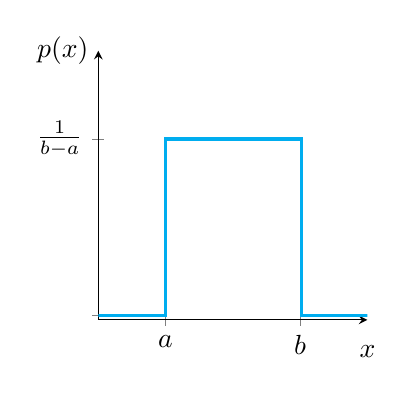
\begin{tikzpicture}[
    declare function={unipdf(\x,\xl,\xu)= (\x>\xl)*(\x<\xu)*1/(\xu-\xl);}
]
\begin{axis}[
    width=5cm,height=5cm,
    xlabel={$x$},
    ylabel={$p(x)$},
    every axis y label/.style={at={(current axis.north west)},left=0mm},
    every axis x label/.style={at={(current axis.south east)},below=2mm},
    width=5cm,height=5cm,
        axis lines=left,
    samples=100,
    const plot mark mid,
    ymin=-0.025,
    ymax=1.5,
    xmin=-0.5,
    xmax=1.5,
    ytick={0, 1},
    yticklabels={ , $\frac{1}{b-a}$},
    xtick={0,1},
    xticklabels={$a$, $b$}
]
\addplot [very thick, cyan] {unipdf(x,0,1)};
\end{axis}
\end{tikzpicture}
\end{document}